\section{Control Flow Graph}\label{control_flow_graph}
If one wants to analyse a program and the analysis is flow sensitive one can use a Control Flow Graph(CFG) to track the flow of the program.
An analysis being flow sensitive means that it does matter in which order pieces of the program are executed.
A CFG is simply just another representation of the program source.
It is a directed graph where a node is a specific place in the program and edges represent the possible options to which the program can execute to.
A CFG always consists of one entry node and one exit node, called \textit{entry} and \textit{exit}.
Given a node \textit{n} the set of predecessor nodes are denoted \textit{pred(n)} and the set of successors are denoted \textit{succ(n)}.

\todo{Ved ikke lige med opsætning af figurer}
We will now look at the control flow structures in the Python programming language.
A CFG for the different control flows for the if statement can be found in \cref{fig:if}.

\begin{figure}
  \centering
  \begin{subfigure}[b]{0.3\textwidth}
    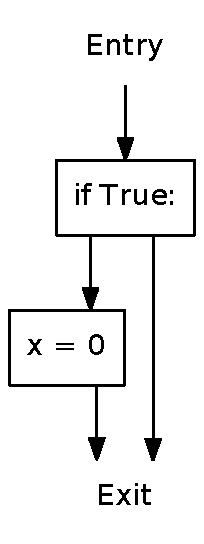
\includegraphics[scale=.5]{./figures/if.pdf}  
    \caption{An if statement.}
    \label{fig:if:if}
  \end{subfigure}
  ~ %add desired spacing between images, e. g. ~, \quad, \qquad, \hfill etc. 
  %(or a blank line to force the subfigure onto a new line)
  \begin{subfigure}[b]{0.3\textwidth}
    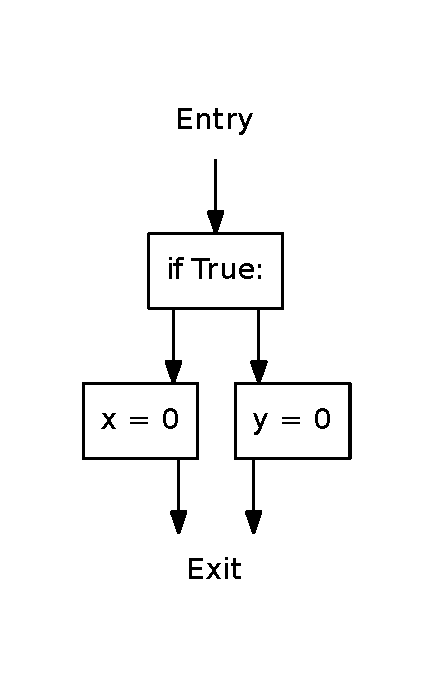
\includegraphics[scale=.5]{./figures/if_else.pdf}
    \caption{An if, else statement.}
    \label{fig:if:if_else}
  \end{subfigure}
  ~ %add desired spacing between images, e. g. ~, \quad, \qquad, \hfill etc. 
  %(or a blank line to force the subfigure onto a new line)
  \begin{subfigure}[b]{0.3\textwidth}
    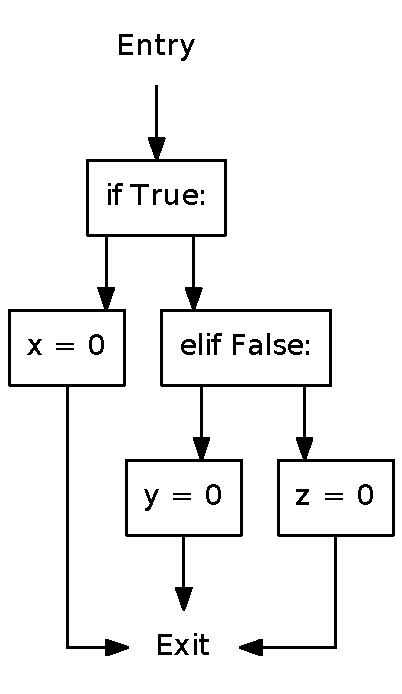
\includegraphics[width=\textwidth]{./figures/if_else_elif.pdf}
    \caption{An if, elif, else statement.}
    \label{fig:if:if_elif_else}
  \end{subfigure}
  \label{fig:if}
\end{figure}

The CFG for the different usage of the while statement can be found in \cref{fig:while}
\begin{figure}
  \centering
  \begin{subfigure}[b]{.4\textwidth}
    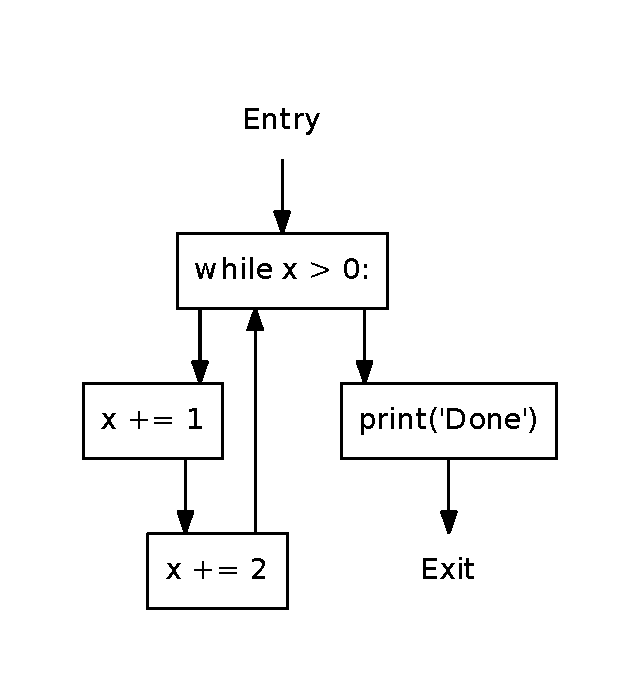
\includegraphics[scale=.5]{./figures/while_no_orelse.pdf}
    \label{fig:while:while_no_orelse}    
    \caption{Simple while statement.}
  \end{subfigure}
  ~
  \begin{subfigure}[b]{.4\textwidth}
    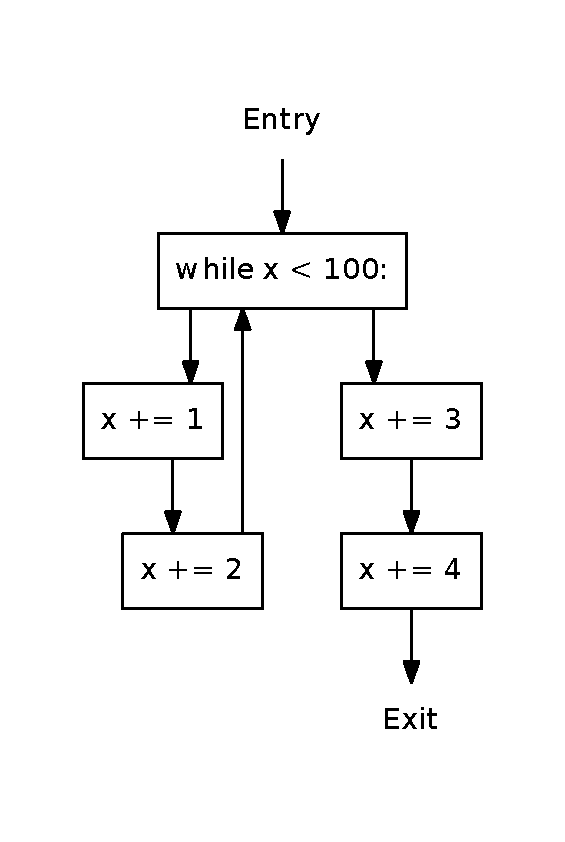
\includegraphics[scale=.5]{./figures/while_else.pdf}
    \caption{While statement with an else clause.}
    \label{fig:while:while_else}
  \end{subfigure}  
  \caption{CFGs of the two different while statements.}
  \label{fig:while}
\end{figure}
